\documentclass[a4paper,12pt]{article}

\usepackage{titlesec}
\setcounter{secnumdepth}{4}
\titleformat{\paragraph}
{\normalfont\normalsize\bfseries}{\theparagraph}{1em}{}
\titlespacing*{\paragraph}
{0pt}{3.25ex plus 1ex minus .2ex}{1.5ex plus .2ex}

%% Language and font encodings
\usepackage[english]{babel}
\usepackage[utf8x]{inputenc}
\usepackage[T1]{fontenc}

%% Sets page size and margins
\usepackage[a4paper,top=3cm,bottom=2cm,left=3cm,right=3cm,marginparwidth=1.75cm]{geometry}

%% Useful packages
\usepackage{amsmath}
\usepackage{mathtools}

\usepackage{amssymb}
\usepackage{graphicx}
\usepackage[colorinlistoftodos]{todonotes}
\usepackage[colorlinks=true, allcolors=blue]{hyperref}
\DeclarePairedDelimiter\set\{\}

\title{Universal simulation of Turing machine in $\mathcal{O}(T\log T)$-time}
\author{Kenenbek Arzymatov}

\begin{document}
\maketitle

\section{Introduction}
\subsection{Turing Machine. }

\textbf{Definition}. Formally, a TM $M$ is described by a tuple $(\Gamma, Q, \delta)$ containing:

\begin{itemize}
\item A finite set  of the symbols that $M$’s tapes can contain. We assume that  contains a
designated “blank” symbol, denoted  $\square$; a designated “start” symbol, denoted  $\rhd$; and
the numbers 0 and 1. We call  the alphabet of M.
\item A finite set $Q$ of possible states $M$’s register can be in. We assume that $Q$ contains a
designated start state, denoted $q_{start}$ , and a designated halting state, denoted $q_{halt}$
\item A function $\delta : Q \times \Gamma^{k} → Q \times \Gamma^{k−1} \times \set*{L, S, R}^{k}$ , where $k ≥ 2$, describing the rules $M$
use in performing each step. This function is called the transition function of $M$.
\end{itemize}

\textbf{Statements}:
\begin{enumerate}
\item Behavior of a Turing machine is determined by its transition function.
\item Every string in $\{0, 1\}^{*}$ represents some Turing machine.
\item Every TM is represented by infinitely many strings.
\end{enumerate}

\textbf{Definition}.We denote by $M_\alpha$ the machine whose representation as a bit string is $\alpha$. An algorithm (i.e., a machine) can be represented as a bit string once we decide on
some canonical encoding.

\textbf{Definition}.The running time is the number of these basic operations performed. We
measure it in asymptotic terms, so we say a machine runs in time $T(n)$ if it performs at
most $T(n)$ basic operations time on inputs of length $n$.

\textbf{Definition}.Let $f : \{0, 1\}^∗ → \{0, 1\}^∗$ and let $T : N → N$ be some functions, and let $M$ be a Turing
machine. We say that M computes $f$ if for every $x ∈ \{0, 1\}∗$ , whenever $M$ is initialized
to the start configuration on input x, then it halts with $f(x)$ written on its output tape.
We say $M$ computes $f$ in $T(n)$-time if its computation on every input $x$ requires at
most $T(|x|)$ steps.

\subsection{EFFICIENCY AND RUNNING TIME}

\textbf{Definition Computing a function and running time}

Let $f : \{0, 1\}^{∗} \rightarrow \{0, 1\}^{*}$ and let $T :  \mathbb{N} →  \mathbb{N}$ be some functions, and let $M$ be a Turing
machine. We say that $M$ computes $f$ if for every $x \in \{0, 1\}^{*}$ , whenever $M$ is initialized
to the start configuration on input $x$, then it halts with $f(x)$ written on its output tape.
We say $M$ computes $f$ in $T(n)$-time if its computation on every input $x$ requires at most $T(|x|)$ steps.

\textbf{Time-constructible functions}

A function $T : \mathbb{N} \rightarrow \mathbb{N}$ is time constructible if $T(n) \geq n$ and there is a TM $M$ that
computes the function $x  \rightarrow  T(|x|)$  in time $T(n)$. (As usual,  $T(|x|)$  denotes the binary
representation of the number $T(|x|).)$ Examples for time-constructible functions are $n, nlogn, n^2 , 2n $. Almost all functions encountered in this book will be time constructible,
and we will restrict our attention to time bounds of this form. (Allowing time bounds
that are not time constructible can lead to anomalous results.) The restriction $T(n) \geq n$
is to allow the algorithm time to read its input.

Most of the specific details of our definition of Turing machines are quite arbitrary. It is
a simple exercise to see that most changes to the definition do not yield a substantially
different model, since our model can simulate any of these new models. In context of
computational complexity, however, we have to verify not only that one model can
simulate another, but also that it can do so efficiently. Now we state a few results of this
type, which ultimately lead to the conclusion that the exact model is unimportant if we
are willing to ignore polynomial factors in the running time. Variations on the model
studied include restricting the alphabet $\Gamma$ to be $\{0, 1, \square, \rhd \}$, restricting the machine to
have a single work tape, or allowing the tapes to be infinite in both directions. All results
in this section are proved sketchily—completing these sketches into full proofs.

\paragraph{Claim}

For every $f : \{0, 1\}^{∗} \rightarrow \{0, 1\}^{*}$ and time-constructible $T :  \mathbb{N} →  \mathbb{N}$ if $f$ is
computable in time $T(n)$ by a TM $M$ using alphabet $\Gamma$, then it is computable in time $4 \log{|\Gamma|}T(n)$ by a TM $\widetilde{M}$ using the alphabet $\{0, 1, \square, \rhd \}$.

\paragraph{Short proof}

Let $M$ be a TM with alphabet $\Gamma$, $k$ tapes, and state set $Q$ that computes
the function $f$ in $T(n)$ time. We describe an equivalent TM $\widetilde{M}$ computing $f$ with alphabet $\{0, 1, \square, \rhd \}$, $k$ tapes and a set $Q'$ of states. The idea behind the transformation is simple:
One can encode any member of $\Gamma$ using $\log |\Gamma|$ bits. Thus, each of $\widetilde{M}$'s work tapes will
simply encode one of $M$’s tapes: For every cell in $M$'s tape we will have log |$\Gamma$| cells in
the corresponding tape of $\widetilde{M}$(see \ref{fig:scetch1}).

\begin{figure}[!ht]
\centering
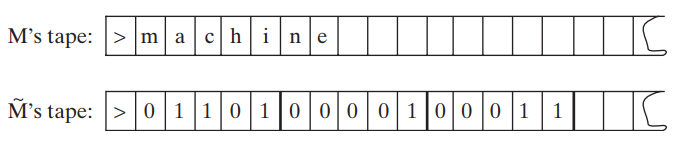
\includegraphics[width=10cm]{scetch1.png}
\caption{We can simulate a machine $M$ using the alphabet $\{\square, \rhd, a, b, ..., z \}$ by a machine $M'$ using $\{0, 1, \square, \rhd \}$ via encoding every tape cell of $M$ using five cells of $M'$.}
\label{fig:scetch1}
\end{figure}

\par	
To simulate one step of $M$, the machine $\widetilde{M}$ will (1) use $\log |\Gamma|$ steps to read from
each tape the $\log |\Gamma|$ bits encoding a symbol of $\Gamma$, (2) use its state register to store the
symbols read, (3) use $M$’s transition function to compute the symbols $M$ writes and $M$'s
new state given this information, (4) store this information in its state register, and (5)
use $\log |\Gamma|$ steps to write the encodings of these symbols on its tapes.
\par 
One can verify that this can be carried out if $\widetilde{M}$ has access to registers that can
store $M$'s state, $k$ symbols in $\Gamma$, and a counter from 1 to $\log |\Gamma|$. Thus, there is such a
machine $\widetilde{M}$ utilizing no more than $c|Q||\Gamma|^{k+1}$ states for some absolute constant $c$. (In
general, we can always simulate several registers using one register with a larger state
space. For example, we can simulate three registers taking values in the sets $A, B \text{ and } C$, respectively, with one register taking a value in the set $A \times B \times C$, which is of size $|A| |B| |C|$.)

\subsection{Oblivious Turing machines}

\paragraph{Claim}
Define a single-tape Turing machine to be a TM that has only one read-write
tape, that is used as input, work, and output tape. For every $f : \{0, 1\}^{∗} \rightarrow \{0, 1\}$ and
time-constructible $T : \mathcal{N} \rightarrow \mathcal{N}$, if $f$ is computable in time $T(n)$ by a TM $M$ using $k$ tapes,
then it is computable in time $5kT(n)^2$ by a single-tape TM  $\widetilde{M}$.

\paragraph{Proof}
Again the idea is simple: The TM $\widetilde{M}$ encodes $k$ tapes of $M$ on a single
tape by using locations $1, k + 1, 2k + 1, ...$ to encode the first tape, locations $2, k +
2, 2k + 2, ...$ to encode the second tape etc. (see Figure \ref{fig:scetch2}). For every symbol a in
$M$'s alphabet, $\widetilde{M}$ will contain both the symbol $a$ and the symbol $a^\wedge$. In the encoding of
each tape, exactly one symbol will be of the "$\wedge$ type", indicating that the corresponding
head of $M$ is positioned in that location (see Figure \ref{fig:scetch2}). $\widetilde{M}$ will not touch the first
$n + 1$ locations of its tape (where the input is located) but rather start by taking $\mathcal{O}(n^2)$
steps to copy the input bit by bit into the rest of the tape, while encoding it in the
above way.

\par 
To simulate one step of $M$, the machine $\widetilde{M}$ makes two sweeps of its work tape: First it sweeps the tape in the left-to-right direction and records to its register the $k$ symbols
that are marked by "$\wedge$". Then $\widetilde{M}$ uses $M$'s transition function to determine the new state,
symbols, and head movements and sweeps the tape back in the right-to-left direction
to update the encoding accordingly. Clearly, $\widetilde{M}$ will have the same output as $M$. Also,
since on $n$-length inputs $M$ never reaches more than location $T(n)$ of any of its tapes, $\widetilde{M}$ will never need to reach more than location $2n + kT(n) \leq (k + 2)T(n)$ of its work tape,
meaning that for each of the at most $T(n)$ steps of $M$, $\widetilde{M}$ performs at most $5 \cdot k \cdot T(n)$
work (sweeping back and forth requires about $4 \cdot k \cdot T(n)$ steps, and some additional
steps may be needed for updating head movement and book keeping). $\blacksquare$

\begin{figure}[!ht]
\centering
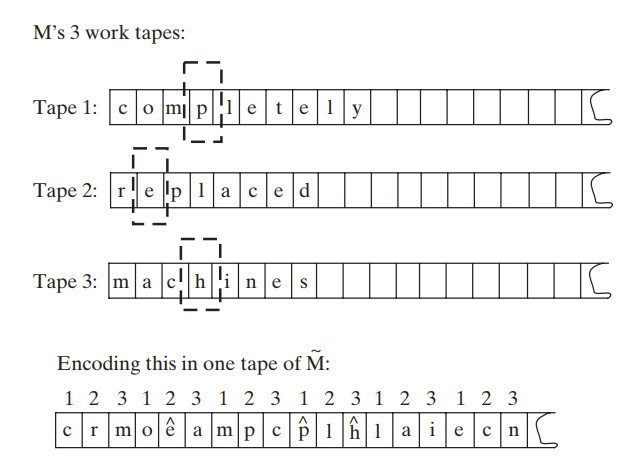
\includegraphics[width=10cm]{s2.png}
\caption{Simulating a machine $M$ with three tapes using a machine $\widetilde{M}$ with a single tape.}
\label{fig:scetch2}
\end{figure}

With a bit of care, one can ensure that the proof of Claim 1.6 yields a TM $\widetilde{M}$ with the following property: Its head movements do not depend on the input but only depend on
the input length. That is, every input $x \in \{0, 1\}^{∗}$ and $i \in \mathcal{N}$, the location of each of $M$’s
heads at the ith step of execution on input $x$ is only a function of $|x|$ and $i$. A machine
with this property is called oblivious, i.e it has following 

\subsection{The universal Turing machine}
\textbf{Definition}.There is a universal Turing machine $U$ that can simulate any other Turing machine given
its bit representation. Given a pair of bit strings $(x, \alpha)$ as input, this machine simulates
the behavior of $M_\alpha$ on input x. This simulation is very efficient: If the running time of
$M_\alpha$ was $T(|x|)$, then the running time of $U$ is $O(T(|x|) \log{T(|x|)})$.
Turing was the first to observe that general-purpose computers are possible, by showing
a universal Turing machine that can simulate the execution of every other TM $M$ given
$M$’s description as input.

But it is
good to remember why it was once counterintuitive. The parameters of the universal
TM are fixed—alphabet size, number of states, and number of tapes. The corresponding
parameters for the machine being simulated could be much larger. The reason this is the ability to use encodings. Even if the universal TM has a
very simple alphabet, this suffices to represent the other machine’s state and transition
table on its tapes and then follow along in the computation step by step.

\subsection{Efficient universal Turing machine}
\subsubsection{Claim}
\textbf{Theorem}.There exists a TM $U$ such that for every $x, \alpha \in \{0, 1\}^{*} , U(x, \alpha) = M_\alpha(x)$, where $M_\alpha$
denotes the TM represented by $\alpha$.
Moreover, if $M_\alpha$ halts on input x within T steps then $U(x, \alpha)$ halts within $CT \log{T}$ steps,
where C is a number independent of $|x|$ and depending only on $M_\alpha$'s alphabet size,
number of tapes, and number of states.

\subsubsection{Proof}
We show a universal $TM \; U$
such that given an input $x$ and a description of a $TM \; M$ that halts on $x$ within $T$ steps,
$U$ outputs $M(x)$ within $\mathcal{O}(T\log T)$ time (where the constants hidden in the $\mathcal{O}$ notation
may depend on the parameters of the $TM \; M$ being simulated).

$U$ will use its input and output
tape in the same way $M$ does and will also have extra work tapes to store $M$’s transition
table and current state and to encode the contents of $M$’s work tapes.

Now we show a way to encode all of M’s work tapes in a single tape of U, which
we call the main work tape of U. 
Let $k$ be the number of tapes that $M$ uses (apart from its input and output tapes)
and  its alphabet. We may assume that $U$ uses the
alphabet $\Gamma^{k}$ (as this can be simulated with a overhead depending only on $k, |\Gamma|$). Thus
we can encode in each cell of $U$’s main work tape $k$ symbols of $\Gamma$, each corresponding
to a symbol from one of $M$'s tapes. This means that we can think of $U$’s main work tape
not as a single tape but rather as $k$ parallel tapes. 

\paragraph{Encoding \texorpdfstring{$M$}{}’s tapes on \texorpdfstring{$U$}{}’s tape}

	We encode the information (the content of $M$'s work tapes) using “buffer zones”: Rather
than having each of $U$’s parallel tapes correspond exactly to a tape of $M$, we add a
special kind of blank symbol $\diamond$ to the alphabet of $U$’s parallel tapes with the semantics
that this symbol is ignored in the simulation.

	For convenience, we think of $U$’s parallel tapes as infinite in both the left and right
directions (this can be easily simulated with minimal overhead: see Claim 1.8). Thus, we
index their locations by $0, \pm 1, \pm 2, \dotsc $. Normally we keep $U$’s head on location 0 of these
parallel tapes. We will only move it temporarily to perform a shift when, following our
general approach, we simulate a left head movement by shifting the tape to the right
and vice versa. At the end of the shift, we return the head to location 0.

	We split each of $U$’s parallel tapes into zones that we denote by
$R_0 , L_0 , R_1 , L_1 , \dotsc$. The cell at location 0 is not at any zone. Zone $R_0$ contains the two cells immediately to the right of location \(C\) (i.e.,
locations \(+1 and +2\)), while Zone \(R_1\) contains the four cells \(+3, +4, +5, +6\). Generally,
for every \(i ≥ 1, \text{Zone} R_i \text{contains the} 2 \cdot 2^i\) cells that are to the right of Zone $R_{i−1}$ (i.e.,
locations \([2 i+1 − 1, . . . , 2 i+2 − 2]\)). Similarly, Zone $L_0$ contains the two cells indexed by
−1 and −2, and generally Zone $L_i$ contains the cells $[−2^{i+2} + 2, \dotsc , −2^{i+1} + 1]$. We
shall always maintain the following invariants:
\begin{itemize}
\item Each of the zones is either empty, full, or half-full with non- 
$\diamond$ is either \(0, 2^i , or 2 \cdot 2^i\) and the same holds
number of symbols in zone $R_i$ that are not 
for $L_i$ . (We treat the ordinary $\square$ symbol the same as any other symbol in $\Gamma$, and in
particular a zone full of  $\square$’s is considered full.) We assume that initially all the zones are half-full. We can ensure this by filling half of each zone with $\diamond$ symbols in the first time we encounter it.
\item The total number of non-$\diamond$ symbols in $R_i \cup L_i$ is $2 \cdot 2 i$. That is, either $R_i$ is empty and $L_i$ is full, or $R_i$ is full and $L_i$ is empty, or they are both half-full.
\item Location 0 always contains a non-$\diamond$ symbol.
\end{itemize}

\paragraph{Performing a shift}
The advantage in setting up these zones is that now when performing the shifts, we do
not always have to move the entire tape, but we can restrict ourselves to only using
some of the zones. We illustrate this by showing how $U$ performs a left shift on the first
of its parallel tapes (see also Figure 1.9):
\begin{enumerate}
\item $U$ finds the smallest $i_0$ such that $R_{i_0}$ is not empty. Note that this is also the smallest $i_0$ such that $L_{i_0}$ is not full. We call this number $i_0$ the $index$ of this particular shift.
\item $U$ puts the leftmost non-$\diamond$ symbol of $R_{i_0}$ in position 0 and shifts the remaining leftmost $2^{i_0} − 1$ non-$\diamond$ symbols from $R_{i_0}$ into the zones $R_0 ,\cdots , R_{i_0 −1}$ filling up exactly half the symbols of each zone. Note that there is exactly room to perform this since all the zones $R_0 ,\cdots , R_{i_0 −1}$ were empty and indeed $2^{i_0}-1 = \sum_{j=0}^{i_0-1} 2^{j}$
\item $U$ performs the symmetric operation to the left of position 0. That is, for $j$ starting from $i_0 −1$ down to 0, $U$ iteratively moves the $2 \cdot 2 j$ symbols from $L_{j+1}$ to fill half the cells of $L_{j+1}$ .Finally, $U$ moves the symbol originally in position 0 (modified appropriately according to $M$’s transition function) to $L_0$.
\item At the end of the shift, all of the zones $R_0 , L_0 , \cdot , R_{i_0 −1} , L_{i_0 −1}$ are half-full, $R_{i_0}$ has $2^{i_0}$ fewer non-$\diamond$ symbols, and $L_i$ has $2^i$ additional non-$\diamond$ symbols. Thus, our invariants are maintained.
\item
The total cost of performing the shift is proportional to the total size of all the zones $R_0 , L_0, R_{i_0} , L_{i_0}$. That is,  $\mathcal{O}( \sum_{j=0}^{i_0} 2 \cdot 2^{j}) = \mathcal{O}(2^{i_0}) operations.$
\end{enumerate}

After performing a shift with index i the zones $L_0 , R_0, L_{i-1} , R_{i-1}$ are half-full,
which means that it will take at least $2^{i − 1}$ left shifts before the zones $L_0, \cdots , L_{i-1}$ become empty or at least $2^{i − 1}$ right shifts before the zones $R_0, \cdots , R_{i-1}$ become
empty. In any case, once we perform a shift with index $i$, the next $2^{i − 1}$ shifts of that
particular parallel tape will all have index less than i. This means that for every one
of the parallel tapes, at most a $1/2^i$ fraction of the total number of shifts have index
$i$. Since we perform at most $T$ shifts, and the highest possible index is $\log T$, the total
work spent in shifting $U$’s k parallel tapes in the course of simulating $T$ steps of $M$ is
$$  \mathcal{O}( k \cdot \sum_{i=1}^{\log T} \frac{T}{2^{i-1}} 2^{i}) = \mathcal{O}(T\log T).\blacksquare $$

\end{document}